\documentclass[crop,tikz]{standalone}
\usepackage{pgfplots}

% http://pgfplots.net/tikz/examples/bell-curve/
\pgfplotsset{compat=1.8}
\pgfmathdeclarefunction{gauss}{2}{\pgfmathparse{1/(sqrt(#2*2*pi))*exp(-((x-#1)^2)/(2*#2))}}
\pgfmathdeclarefunction{multigauss}{4}{\pgfmathparse{1/(sqrt(#2*2*pi))*exp(-((x-#1)^2)/(2*#2)) * 1/(sqrt(#4*2*pi))*exp(-((y-#3)^2)/(2*#4))}}

\pgfplotsset{colormap={whiteblack}{color(0cm)=(white); color(1cm)=(gray)}}

\usetikzlibrary{positioning,shapes,arrows}

\begin{document}
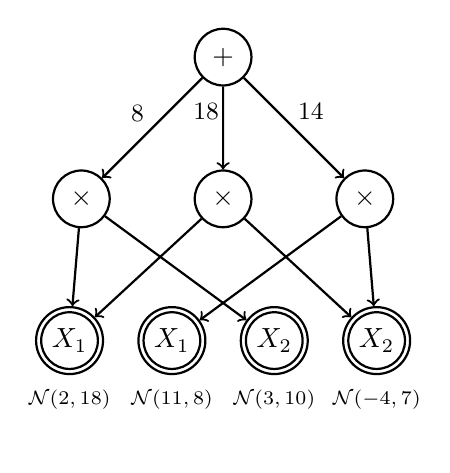
\begin{tikzpicture}
    [scale=.6,auto=left,every node/.style={draw, thick, circle, inner sep = 0pt, minimum width = 0.72cm}]
  \node (n1) at (5,10) {$+$};
  \node (n2) at (2,7) {$\times$};
  \node (n3) at (5,7) {$\times$};
  \node (n4) at (8,7) {$\times$};
  \node (n5) at (1.75,4) {$X_1$};
  \node (n6) at (3.9166,4) {$X_1$};
  \node (n7) at (6.0833,4) {$X_2$};
  \node (n8) at (8.25,4) {$X_2$};

  \node[minimum width = 0.85cm] (n5) at (1.75,4) {};
  \node[minimum width = 0.85cm] (n6) at (3.9166,4) {};
  \node[minimum width = 0.85cm] (n7) at (6.0833,4) {};
  \node[minimum width = 0.85cm] (n8) at (8.25,4) {};

  \node[draw=none] (n9) at (1.75,2.75) {\scriptsize $\mathcal{N}(2, 18)$};
  \node[draw=none] (n10) at (3.9166,2.75) {\scriptsize $\mathcal{N}(11, 8)$};
  \node[draw=none] (n11) at (6.0833,2.75) {\scriptsize $\mathcal{N}(3, 10)$};
  \node[draw=none] (n12) at (8.25,2.75) {\scriptsize $\mathcal{N}(-4, 7)$};

  \foreach \from/\to/\weight/\pos in {n1/n2/$8$/above left, n1/n3/$18$/above left, n1/n4/$14$/above right}
    \draw (\from) edge[->, thick] node[\pos, draw=none, circle=none, minimum width=0.5cm, minimum height=0.2cm, inner sep=2pt]{\small \weight} (\to);

  \foreach \from/\to in {n2/n5, n2/n7, n3/n5, n3/n8, n4/n6, n4/n8}
    \draw (\from) edge[->, thick] (\to);
\end{tikzpicture}
\end{document}
